\documentclass[12pt]{article}
\usepackage{url,graphicx,tabularx,array}
\usepackage[margin=1in]{geometry}
\setlength{\parskip}{1ex} %--skip lines between paragraphs
\setlength{\parindent}{0pt} %--don't indent paragraphs

\usepackage{algorithmic}
\usepackage{algorithm}
\usepackage{ amssymb }
\usepackage{ latexsym }
\usepackage{ amsmath }
\usepackage{ amsthm }
%-- Commands for header
\renewcommand{\title}[1]{\textbf{#1}\\}
\renewcommand{\line}{\begin{tabularx}{\textwidth}{X>{\raggedleft}X}\hline\\\end{tabularx}\\[-0.5cm]}
\newcommand{\leftright}[2]{\begin{tabularx}{\textwidth}{X>{\raggedleft}X}#1%
& #2\\\end{tabularx}\\[-0.5cm]}

\newtheorem{defn}{Definition}[section]
\newtheorem{conjecture}{conjecture}[section]
\newtheorem{lemma}{Lemma}[section]
\newtheorem{corollary}{Corollary}[section]
\newtheorem{question}{Question}[section]
\newtheorem{proposition}{Proposition}[section]


%\linespread{2} %-- Uncomment for Double Space
\begin{document}

\title{Homework 6: CMPS 242}
\line
\leftright{\today}{Bryan Matsuo (bmatsuo@soe.ucsc.edu) \& John St. John (jstjohn@soe.ucsc.edu)} %-- left and right positions in the header
\begin{enumerate}
\item \textbf{AdaBoost:}



\item \textbf{T base learners:}

Let $C_t \in \{0,1\}$ be  the event that learner $t$ predicts correctly. All $C_t$ are independent, and the $\Pr(C_t=1) = p$. The majority prediction of the learners is correct is $\sum_{t=1}^TC_t > \left\lfloor \frac{T}{2} \right\rfloor $. Because $C_t$ is a Bernoulli random variable, their sum is a binomial with parameters $T$ and $p$. The probability of a correct majority of votes becomes $1-F\left(\left\lfloor\frac{T}{2}\right\rfloor\right)$ where $F(x)$ is the CDF of a binomial with parameters $T$ and $p$. 
\begin{equation}
\Pr(\text{Correct Majority}) = 1- \sum_{k=0}^{\left\lfloor T/2 \right\rfloor} {T \choose k}p^k(1-p)^{T-k}
\end{equation}

\begin{figure}[htbp]
\begin{center}
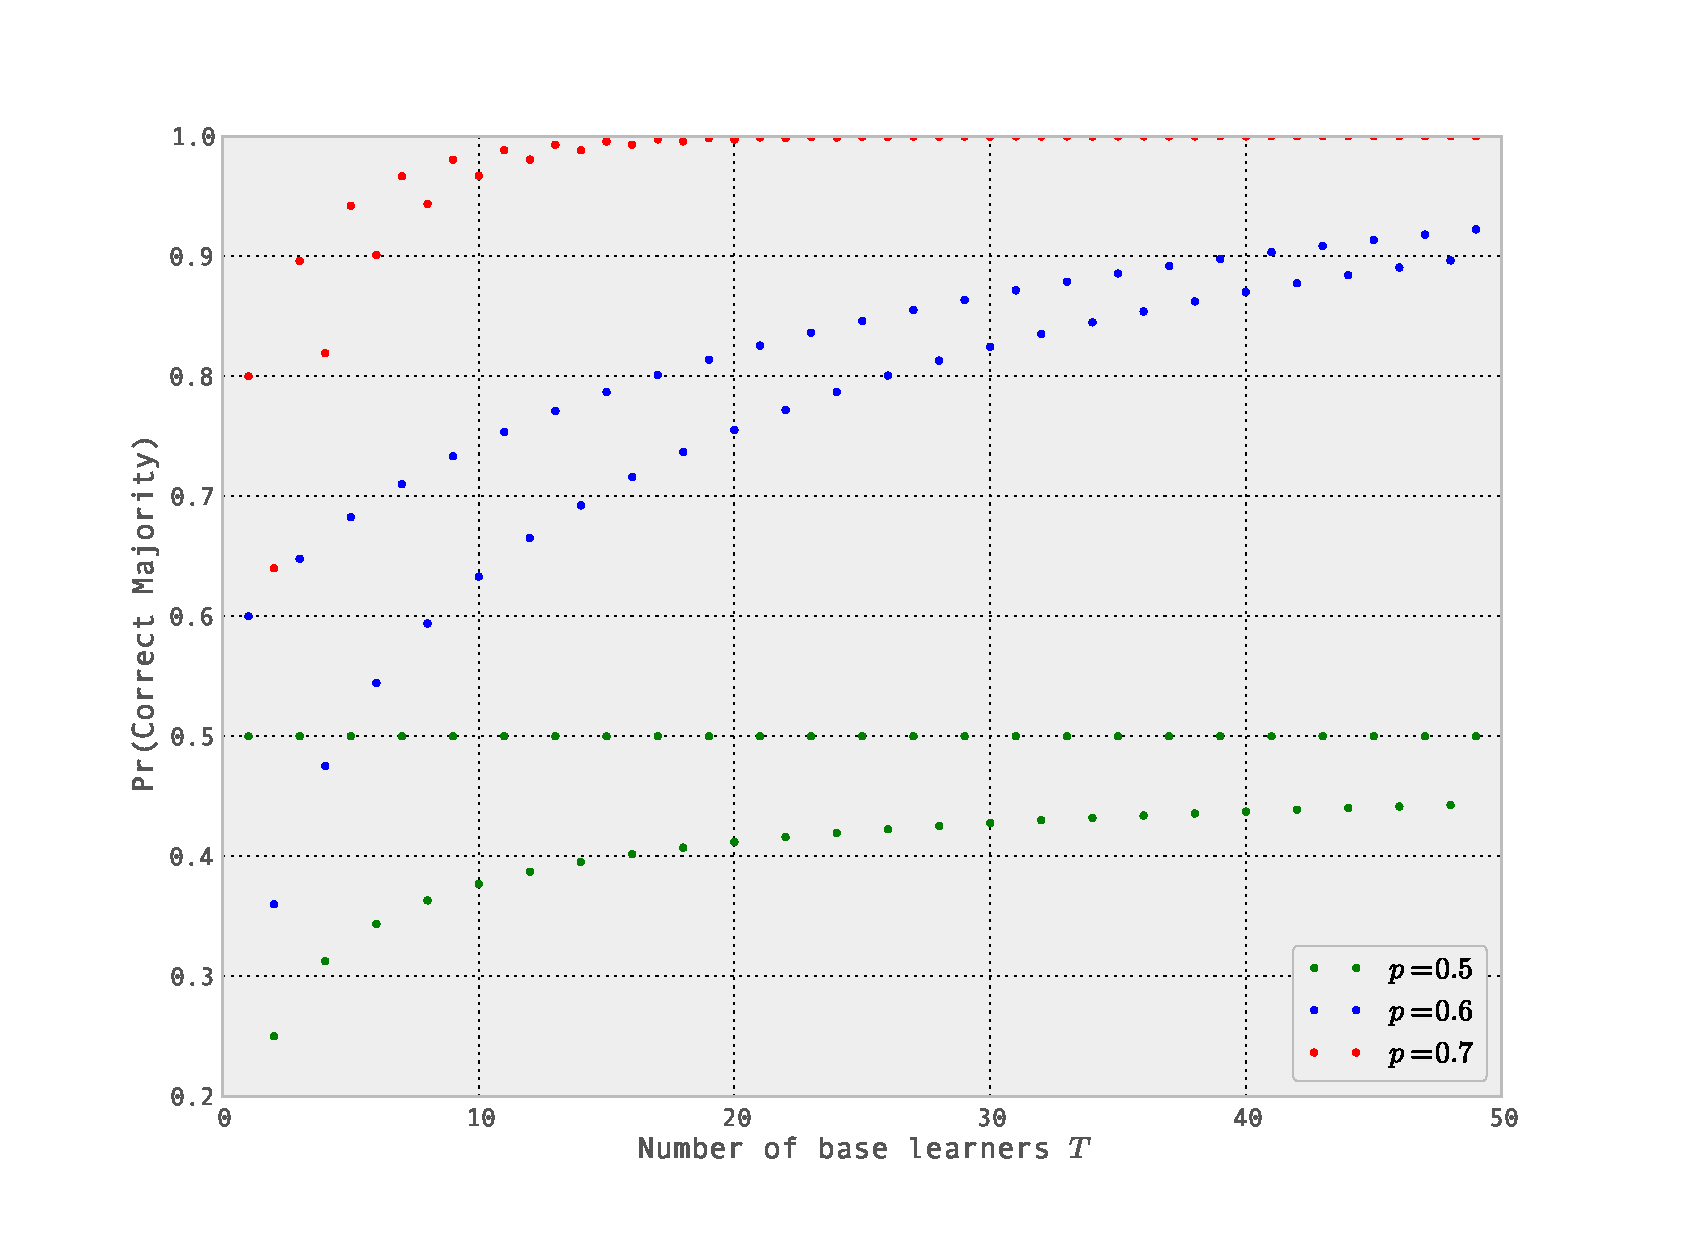
\includegraphics{prob2.eps}
\caption{Plot of probability of voting, given different probabilities of votes, and numbers of voters.}
\label{fig:prob2}
\end{center}
\end{figure}


\item \textbf{EM Clustering:}

Since each of the gaussians share all of the points with the same weight, they start off exactly the same. Since the update does not incorporate a randomizer, and each of the gaussians are updated in one step, they will all be updated deterministically in the same way. This means they will always be the same gaussians.

\end{enumerate}
\end{document}
